\documentclass[10pt]{article}

\usepackage{amsmath}

\numberwithin{equation}{section}

\usepackage[english]{babel}
\usepackage[utf8]{inputenc}
\usepackage{amsfonts}
\usepackage{graphicx}
\usepackage{epstopdf}
\usepackage{caption}
\usepackage{float}
\usepackage{bm}
\usepackage{esvect}
\usepackage{hyperref}
\usepackage{listings}

\usepackage{setspace}
\onehalfspacing

\oddsidemargin = 5pt
\evensidemargin = 5pt
\textwidth = 400pt
\topmargin = 5pt
\textheight = 600pt

\title{SPM Report}
\date{}
\author{
	Massimo Equi\\
	AY 2017/2018
}

\begin{document}
\maketitle

\section{Introduction}  \label{intro}
The chosen project is the one consisting in using a genetic algorithm to estimate an unknown function $f$ given a set of pairs $\left(x, f\left(x\right)\right)$ as input.

\section{User Manual} \label{usermanual}
In order to compile and run the program follow these instructions:
\begin{itemize}
\item move to the \verb|SPM_FinalProject| directory;
\item (if a previous pair of \verb|main.out| and \verb|parallel_main.out| files is present) run the command \verb|make clean|; 
\item compile the program with the command \verb|make -f [makefile]|
\item run the sequential program with \verb|./main.out [parameters] < [input_file]|
\item run the parallel program with \verb|./parallel_main.out [parameters] < [input_file]|
Here it is an example of a typical session:
\begin{verbatim}
$ make clean
$ make -f Makefile.icc
$ make -f Makefile.parallel.icc
$ ./main.out 12000 5 4000 10 20 0.5 no < input_cos\(x\)-pow\(x,3\)10-3.txt
$ ./parallel_main.out 12000 5 4000 10 20 0.5 8 no < input_cos\(x\)-pow\(x,3\)10-3.txt
\end{verbatim}
\paragraph{Makefile}
There are several Makefiles to compile the program with different options and compilers. For compiling the sequential program, \verb|[makefile]| can be one of the following:
\begin{itemize}
	\item \verb|make -f Makefile| (or simply \verb|make|) compiles the program with the \verb|g++| compiler;
	\item \verb|make -f Makefile.icc| compiles the program with the \verb|icc| compiler;
	\item \verb|make -f Makefile.icc.mic| compiles the program with the \verb|icc| compiler using the flag \verb|-mmic|;
\end{itemize}
All of the above commands output a \verb|main.out| file.\\
For compiling the parallel program instead use the following in place of \verb|[makefile]|:
\begin{itemize}
	\item \verb|make -f Makefile.parallel| compiles the program with the \verb|g++| compiler;
	\item \verb|make -f Makefile.parallel.icc| compiles the program with the \verb|icc| compiler;
	\item \verb|make -f Makefile.parallel.icc.mic| compiles the program with the \verb|icc| compiler using the flag \verb|-mmic|;
\end{itemize}
All of the above commands output a \verb|parallel_main.out| file.
\paragraph{Run the program}
The program runs with several parameters and has to be called with and input file. Calling \verb|./main.out| or \verb|./parallel_main.out| with no arguments will show a quick guide. \verb|[parameters]| consists in the following: 
\begin{itemize}
	\item \verb|tree_no| is the number of trees that will be created in the random pool generated at the beginning of every execution;
	\item \verb|depthmax| is the maximum possible depth a tree in the pool can have;
	\item \verb|threshold| is the number of trees the algorithm will select to generate the next population (has to be lesser than \verb|tree_no|);
	\item \verb|randmax| is the largest value a leaf of a tree holding a constant can have;
	\item \verb|gen_no| is the number of generations such that, once reached, the algorithm will terminate;
	\item \verb|err| is the threshold for the fitness. If the fitness of the best tree is lesser that \verb|err| the program will terminate; if \verb|err| is a negative number the algorithm will stop only after reaching \verb|gen_no| generations;
	\item \verb|nw| is the number of parallel workers (skip this argument if the program is sequential);
	\item \verb|debug| can be either \verb|yes| or \verb|no|; if it is \verb|yes| it runs the program with detailed information at each generation.	   
\end{itemize}
The program requires an input file to run. Any file in this project root directory whose name begins with the string \verb|input_| is a legal input file. In all the executions mentioned in this report we used the input file \verb|input_cos(x)-pow(x,3)10-3.txt| (\verb|10-3| in the name of the file means there are $10^3$ input pairs $(x,f(x))$ in that file).\\
After having compiled the main program, the command \verb|make [makefile] test| can be used to generate the \verb|test_FitnessTime.out|. This little test program can be executed specifying an input file (and no arguments) in order to get some estimations about the time needed to evaluate a tree and compute the fitness 	function.
\end{itemize}

\section{Structure of the code} \label{codestructure}
The code has two main directories: \verb|src/| is where the \verb|.cpp| source files are located while \verb|include/| is where the \verb|.h| header files can be found. Both \verb|src/| and \verb|include/| are structured in three subdirectories: \verb|grammar/|, \verb|genetics/| and \verb|main/|.

\paragraph{grammar}
In \verb|grammar/| there are all the classes needed to implement the grammar provided in the project assignment. Every class is implementing a nonterminal symbol of the grammar with methods that allows it to be expanded using one of its production. The nonterminal \verb|<unop>| and \verb|<binop>| are directly encapsulated in the class \verb|Node| which of course implement the nonterminal \verb|<node>|. Each of these classes gives a concrete implementation of the abstract class \verb|INode|, which is meant to represent a generic node in the syntax tree. An object of class \verb|Node| can be randomly expanded to a given depth using the method \verb|Node::expandRandom()|. Finally, the parameter \verb|randmax| gives and upper bound to the highest number that the class \verb|Const| can store.

\paragraph{genetics}
In \verb|genetics/| the class \verb|Tree| is implementing the behavior of a syntax tree meant to represent a function. Basically, \verb|Tree| provides a nice interface to store and manage the root node of this syntax tree. Indeed, such syntax tree will be generated calling the \verb|Node::expandRandom()| method of that root node. The class \verb|Forest| is the core of the algorithm since it manages a pool of \verb|Tree|s providing methods to perform mutation and crossover over them. The \verb|ParallelForest| class is a subclass of \verb|Forest| and it is used to override the part of the code that was chosen to be turned from sequential to parallel.

\paragraph{main}
In \verb|main/| the file \verb|evolution_cyle.hpp| uses a \verb|Forest| to implement the genetic algorithm. \verb|main.cpp| and \verb|parallel_main.cpp| call \verb|evolution_cycle.hpp| passing it respectively either a \verb|Forest| or a \verb|ParallelForest|.

\section{Parallelization Choices}
\subsection{Decomposition Strategy}
The main operations that our algorithm is performing are: \emph{selection}, \emph{mutation} and \emph{crossover}, \emph{replication}. Running the sequential version of the program we see that the completion time of \emph{selection} is usually two orders of magnitude larger than the one needed for \emph{replication}, \emph{mutation} and \emph{crossover}. Thus, we focus only on optimizing \emph{selection} since, for this reason, that is the crucial issue.\\
Analyzing the structure of the problem we observe that it is embarrassingly parallel at two different level of grain. At each iteration our program has to compute the fitness function of all the trees in our pool, hence for every of those trees it is required to evaluate the function that tree is representing over all input data points. This means we could parallelize:
\begin{itemize}
	\item at a \textbf{fine grain} level, evaluating in parallel the function represented by a single tree over different data points;
	\item at a \textbf{coarse grain} level, computing in parallel the fitness function for different trees.
\end{itemize}
Therefore, the first thing we have to discuss if it is worth it to parallelize at any of this two levels of grain.
\paragraph{Single tree parallelization}
In a typical execution of the code we have to handle trees whose depth is set to be not greater that $8$. This is because most of the times the best trees tent to be the shallower ones hence it is useless to set a very high depth since the deeper trees most probably will be discarded soon. Moreover, the average depth is usually smaller than $3$; this means that on the average we perform $2^{3+1}-1=15$ floating point operations per tree, assuming a floating point operation per node. This means that the amount of time we spend evaluating a tree has roughly at most $10^{-1}\mu$$s$ order of magnitude. If we compare this with the time spent to create a thread (approximately $10\mu$$s$) we realize that even if every worker of our hypothetical parallel computation processed $100$ input points this would still be comparable with the effort needed to set up the thread for that worker, hence at least $1000$ input points per thread are needed to have a reasonable advantage. Therefore, if for instance we supposed to work with $10$ workers, we would need more that $10^{4}$ input points to get any advantage from the parallelization, and this would rarely be the case. This is clearly a scenario where we would have a very poor scalability. Thus, we conclude claiming that it is not worth it to parallelize the program relaying on such a fine grain.
\paragraph{Pool parallelization}
Considering instead the whole pool of trees the workload that would be assigned to a worker in a parallel computation is reasonably large and, more importantly, increases easily with the input size. The fitness function for a tree is computed in order of $10^{2}\mu$$s$, hence having only $10$ trees per worker is already enough to get a workload of $10^{3}\mu$$s$. Typically we work with a pool consisting of thousands of trees and this usually means that every worker will have order of $10^{2}$ trees to handle, even in situations with hundreds of parallel workers. Hence we conclude that is worth it to parallelize at this level of grain.

\subsection{Implementation of the Parallel Part of the Code}
The difference between the sequential and the parallel version of the code resides in the class \verb|ParallelForest|. This class has two additional instance variables: \verb|nw| specifies the number of workers to be used for the parallel computation; \verb|pf| is an unique pointer to a \verb|FastFlow ParallelFor| object. \verb|ParallelForest| overrides the \verb|Forest::fitness()| method, replacing the \verb|C++| sequential \verb|for| loop with the \verb|FastFlow pf->parallel_for()| function, called with the \verb|ParallelForest::nw| parameter. We could use a parallel for due to the fact that no synchronization is needed among the various iterations of the loop since computing the fitness function resembles the \emph{map} pattern.

\section{Expected Results}
We want to be able to express our results in terms of \emph{speedup}, \emph{scalability} and \emph{efficiency}, hence the first thing we need to know is the running time of the sequential program. We ran the sequential program on the Xeon machine $12$ times with these parameters:
\begin{verbatim}
	tree_no = 12000; depthmax = 5; threshold = 4000;
	randmax = 10; gen_no = 20; err = -1.
\end{verbatim}
Removing the most outstanding outliers and taking the average we got a sequential completion time of $T_{seqXeon} =  28.62564 s$. For the Xeon PHI we followed the same procedure for performing the measurements but we decided to use a smaller set of trees since the clock speed of this machine is significantly slower. We therefore used:
\begin{verbatim}
	tree_no = 2400; depthmax = 5; threshold = 800;
	randmax = 10; gen_no = 20; err = -1;
\end{verbatim}
and we got this sequential completion time: $T_{seqPHI} = 60.10967$.\\
In our scenario we have parallelized our code using a farm pattern whose overheads resides mostly on splitting the initial task in several subtasks and assigning them to different parallel executors. This splitting-and-assigning phase has to be performed at the beginning of each iteration of the evolution cycle, hence could potentially lead to a substantial overhead\\
What we expect to get is a speedup that grows steadily with the growing of the parallel executors. In particular, we would like to at least halve the completion time with already $2$ to $6$ workers and to almost achieve the best completion time with $10$ to $12$ workers. As a consequence, we expect to have a speed up closer to the ideal one using up to $6$ workers and then to have it grow slower. Additionally, an ideal speedup would imply the following ideal completion times:
\begin{align}
	T_{par\left(2\right)} &= \frac{T_{seqXeon}}{2} = 14.31282s\\
	T_{par\left(4\right)} &= \frac{T_{seqXeon}}{4} = 7.15641s\\
	T_{par\left(6\right)} &= \frac{T_{seqXeon}}{6} = 4.77094s
\end{align}
Assuming that roughly $frac{1}{10}$ of the sequential completion time is related to the part of the code which remains serial also in the parallel version (\emph{mutation} and \emph{crossover} time plus \emph{replication} time) we will effectively parallelize the $\frac{9}{10}$ of that time. Considering that we will also pay for some overhead, realistically the completion times could be the followings:
\begin{align}
	T_{par\left(2\right)} &= \frac{\frac{9}{10} T_{seqXeon}}{2} + \frac{1}{10} T_{seqXeon} + overhead = 15.744102s + overhead\\
	T_{par\left(4\right)} &= \frac{\frac{9}{10} T_{seqXeon}}{4} + \frac{1}{10} T_{seqXeon} + overhead = 9.30333s + overhead\\
	T_{par\left(6\right)} &= \frac{\frac{9}{10} T_{seqXeon}}{6} + \frac{1}{10} T_{seqXeon} + overhead = 7.15641s + overhead
\end{align}
For the Xeon PHI machine we expect indeed to have a good scalability since the clock speed is lower and even a small amount of trees per worker, say $100$, could be a reasonable workload.

\section{Achieved Results}
Here we report the actual completion times we measured on the Xeon CPU E-2650 and the Xeon PHI machines for the parallel executions of the program, alongside with the graphs for the \emph{speedup}, \emph{scalability} and \emph{efficiency}, comparing these results with the sequential program's ones. The \verb|err| parameter has been always set to \verb|-1| in order to perform exactly \verb|gen_no| iterations; we would not have been able to have comparable results otherwise.
\paragraph{Format of the results}
The program uses \verb|std::chrono| statements in order to outputs the time spent to perform the computation. We stored all the results in two files: the file \verb|tests| for the Xeon machine and the file \verb|tests.phi| for the Xeon PHI machine. Both files has a line storing the output of the \verb|uptime| command in order to record the state of the machine at the execution time. Each one of the lines storing the results of the tests starts with the string \verb|results|, hence you can get the list of all the outputs with the command \verb|grep results tests[.phi]|. \verb|tests| has been produced recording the output on the shell via a \verb|script| command while for \verb|tests.phi| we just used output redirection (since there is no command \verb|script| on the Xeon PHI). The scripts \verb|test.sh| and \verb|test.phi.sh| run all the tests from scratch (without recording them by their own), but this requires a huge amount of time and we think it will not be needed.
\paragraph{Gathering the results}
Certainly, in order to have comparable measures and to compute \emph{speedup}, \emph{scalability} and \emph{efficiency}, we used the same parameter setting we had for the sequential execution and we repeat it here for the seek of readability. Thus, for the \textbf{Xeon} we had:
\begin{verbatim}
	tree_no = 12000; depthmax = 5; threshold = 4000;
	randmax = 10; gen_no = 20; err = -1;
	nw = [1, 2, 4, 6, 8, 10, 12, 14, 16];
\end{verbatim}
while for the \textbf{Xeon PHI} we had:
\begin{verbatim}
tree_no = 2400; depthmax = 5; threshold = 800;
randmax = 10; gen_no = 20; err = -1;
nw = [1, 10, 20, 30, 40, 50, 60, 70, 80, 90, 100, 110, 120].
\end{verbatim}
We passed \verb|input_cos(x)-pow(x,3)10-3.txt| as input file, hence we had $1000$ input pairs $(x, f(x))$. As previously stated, the smaller number of trees on the Xeon PHI is due to the lower clock speed. Since our program is very flops-intensive and the Xeon PHI has $120$ ALU, we did not test with more than $120$ workers for avoiding not to have a true parallelism. Both in the sequential and parallel case we performed $12$ runs of the program, we took out the two most outstanding completion time outliers and then we computed the average of the remaining. 

\subsection{Xeon}
Has we can see from the graphs, the completion time is not as good as it was supposed to be. Indeed, in the formula we gave for a realistic parallel completion time we left the variable $"overhead"$ to capture the fact that we had still to exactly quantify how much time it is required to dispatch the workload to the various workers. Considering for instance $T_{par\left(2\right)}$ we see that now we get a real value of $22.89348s$, implying that we should have $overhead = 22.89348s - 15.744102s = 7.149378s$. This seems to suggest that the overhead is still to high and would explain why we got such a poor speedup (as showed in the graphs). Another possible explanation could be that the compiler is able to perform some optimizations for the sequential program that are not possible with the parallel one, although we do not think this is the case since the completion time for one worker $T_{par\left(1\right)}$ is more or less the same of the sequential one.
\subsection{Xeon PHI}
Even in this case we experience the same issue as for the Xeon. Here we got better results in terms of speedup, passing from a completion time of $~58s$ using $1$ worker to $~4s$ with $10$ workers. The problem is that the poor scalability: the performances go worse with the growing of the number of workers we use. Due to this behavior (high boost with fewer workers, little improvements with more of them) we believe that the input size has really been an issue and it would be interesting to run the tests again with a larger pool of trees. We chose such a pool size for our measurements because a larger one would require much more time to complete all the tests.

\begin{figure} 
	\centering
	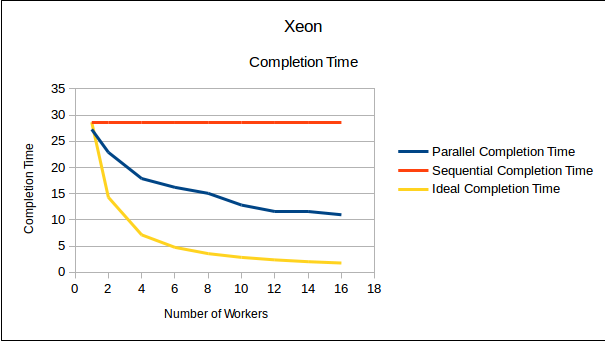
\includegraphics[scale=.75]{Xeon_CompletionTime.png}
	\label{fig:xeoncompletiontime}
\end{figure}

\begin{figure} 
	\centering
	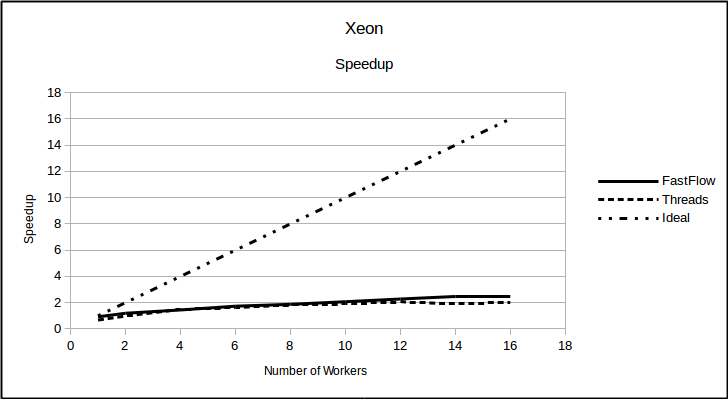
\includegraphics[scale=.75]{Xeon_Speedup.png}
	\label{fig:xeonspeeduptime}
\end{figure}

\begin{figure} 
\centering
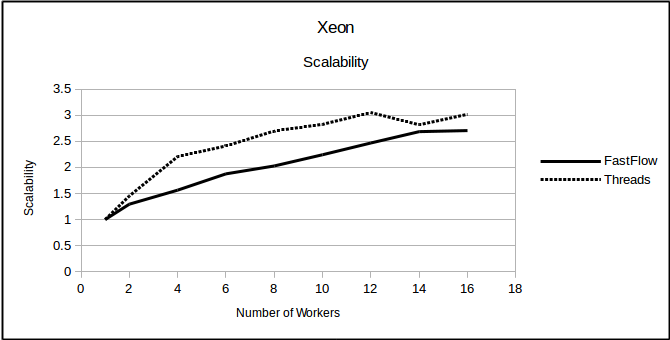
\includegraphics[scale=.75]{Xeon_Scalability.png}
\label{fig:xeonscalability}
\end{figure}

\begin{figure} 
\centering
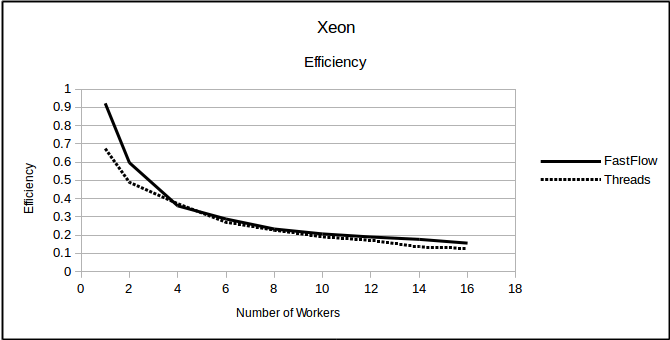
\includegraphics[scale=.75]{Xeon_Efficiency.png}
\label{fig:xeonefficiency}
\end{figure}

\begin{figure} 
	\centering
	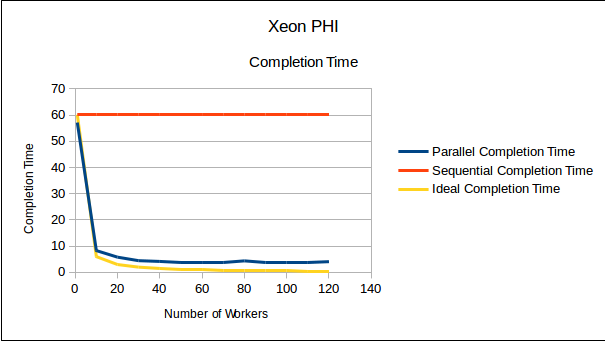
\includegraphics[scale=.75]{XeonPHI_CompletionTime.png}
	\label{fig:xeonphicompletiontime}
\end{figure}

\begin{figure} 
	\centering
	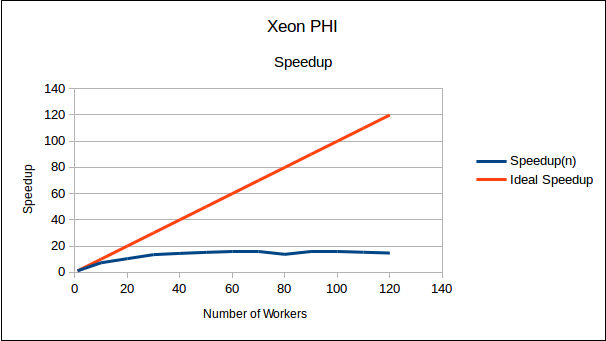
\includegraphics[scale=.75]{XeonPHI_Speedup.png}
	\label{fig:xeonphispeeduptime}
\end{figure}

\begin{figure} 
	\centering
	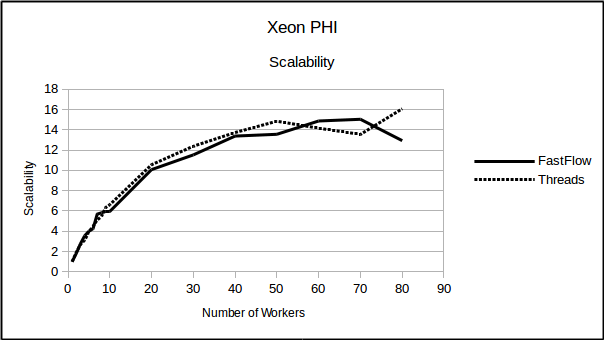
\includegraphics[scale=.75]{XeonPHI_Scalability.png}
	\label{fig:xeonphiscalability}
\end{figure}

\begin{figure} 
	\centering
	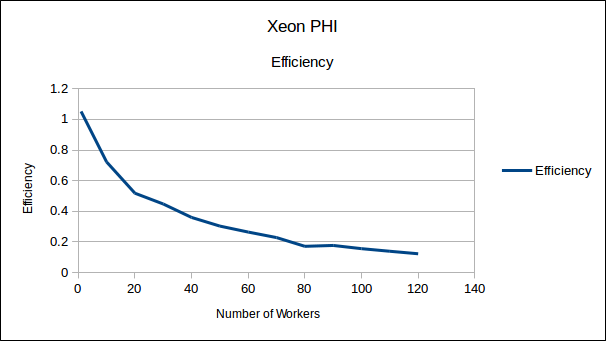
\includegraphics[scale=.75]{XeonPHI_Efficiency.png}
	\label{fig:xeonphiefficiency}
\end{figure}

\end{document}

